\documentclass[10pt,a4paper]{article} %
\usepackage[utf8]{inputenc} %
\usepackage[margin=2cm]{geometry} %
\usepackage[table,xcdraw]{xcolor} %
\usepackage{acronym} %
\usepackage{tikz} %
\usepackage{enumitem} %
\usepackage[binary-units=true,per-mode=repeated-symbol]{siunitx} %
\usepackage{multirow} %
\usepackage{textcomp} %
\usepackage{multirow} %
\usepackage{soul} %
\usepackage{ifthen} %
\usepackage{subcaption} %
\usepackage{hyperref} %
\usepackage{microtype} %
\usepackage{natbib} %
%
\captionsetup{labelfont=bf} %
\captionsetup{font=footnotesize} %
\captionsetup{skip=5pt} %
%
\usetikzlibrary{calc,decorations.pathreplacing,angles,quotes} %
%
\DeclareSIUnit\transfer{T} %
%
\setlength{\bibsep}{4pt} %
%
\title{ %
    \textbf{Assessing On-Chip High-Performance Interfaces on Xilinx and Intel \acs{FPGA}-\acs{SoC} Devices}\\ %
    \textit{Reconfigurable Computing 2019/2020} %
} %
\author{João Vieira} %
\date{\today} %
%
\renewcommand*\acffont{\emph} %
\renewcommand*\acfsfont{\emph} %
%
\acrodef{SoC}{System on Chip} %
\acrodefplural{SoC}{Systems on Chip} %
\acrodef{CPU}{Central Processing Unit} %
\acrodef{FPGA}{Field-Programmable Gate Array} %
\acrodef{PCI}{Peripheral Component Interconnect} %
\acrodef{DMA}{Direct Memory Access} %
\acrodef{GP}{General-Purpose} %
\acrodef{F2H}{\acs{FPGA}-to-\acs{HPS}} %
\acrodef{F2S}{\acs{FPGA}-to-SDRAM} %
\acrodef{HP}{High-Performance} %
\acrodef{FIFO}{First-In-First-Out} %
\acrodef{ACP}{Accelerator Coherency Port} %
\acrodef{HPS}{Hard Processor System} %
\acrodef{PS}{Processing System} %
\acrodef{PL}{Programmable Logic} %
\acrodef{GPU}{Graphic Processing Unit} %
\acrodef{RTL}{Register Transfer Level} % 
\acrodef{VHDL}{VHSIC Hardware Description Language} %
\acrodef{ASIC}{Application Specific Integrated Circuit} %
\acrodef{FSM}{Finite-State Machine} %
\acrodef{MSGDMA}{Modular Scatter-Gather Direct Memory Access} %
\acrodef{ALM}{Adaptive Logic Module} %
\acrodef{BRAM}{Block RAM} %
\acrodef{DSP}{Digital Signal Processing} %
\acrodef{LUT}{Look-Up Table} %
\acrodef{FF}{Flip-Flop} % %
%
\begin{document} %
%
\maketitle %
%
\begin{abstract} %
    \acp{SoC} are devices that include several circuits with different functionalities cooperating to perform a given computational workload. For instance, Xilinx and Intel produce \acp{SoC} that integrate both hard \acp{CPU} and \acp{FPGA}, communicating through on-chip high-performance interfaces. Such interfaces usually allow for much higher data rates than off-chip connections, such as \ac{PCI}, and also lower latencies. The work proposed in this document aims at assessing the performance of the communication channels between the \acp{CPU} and the \ac{FPGA} fabric of two \ac{SoC} devices produced by Xilinx and Intel. The obtained performance measurements are compared with the theoretical bandwidth of the devices as advertised by the producing brands, and the methodology for reproducing the results is briefly explained. %
\end{abstract} %
% 
\acresetall %
%
\section{Introduction}

\ac{FPGA}-based \acp{SoC}, also called \ac{FPGA}-\acp{SoC}, are devices that combine hard \acp{CPU} with reconfigurable logic. Such devices are useful for executing workloads that can benefit from hardware acceleration without resourcing to power-hungry \acp{GPU} or fabricating custom \acp{ASIC}.

\begin{table}[!b] %
    \centering
    \caption{On-chip interface comparison between the Xilinx ZYNQ-7000 and the Intel Cyclone V device families.}
    \label{tab:interface_summary}
    \begin{tabular}{|c|c|}\hline %
        \textbf{Xilinx ZYNQ-7000} & %
        \textbf{Intel Cyclone V} \\\hline %
        %
        \parbox{.47\linewidth}{ %
            \vspace{1mm} %
            \textbf{\acf{GP} ports:} There are two of these ports in the ZYNQ-7000 devices. They have a fixed width of \SI{32}{\bit} and no internal buffers, making them suitable for low-throughput applications. %
            \vspace{1mm} %
        } & %
        \parbox{.47\linewidth}{ %
            \vspace{1mm} %
            \textbf{\acf{F2H}:} This port has a configurable width of 32, 64 or \SI{128}{\bit}. Being suitable for lightweight communication, it resembles the \ac{GP} ports of the ZYNQ-7000 devices. %
            \vspace{1mm} %
        } \\\hline %
        %
        \parbox{.47\linewidth}{ %
            \vspace{1mm} %
            \textbf{\acf{HP} ports:} There are four of these ports in the ZYNQ-7000 devices. They have widths of either 32 or \SI{64}{\bit} and built-in \acp{FIFO}, making them suitable for high throughput applications. %
            \vspace{1mm} %
        } & %
        \parbox{.47\linewidth}{ %
            \vspace{1mm} %
            \textbf{\acf{F2S}:} Instead of offering four ports like the ZYNQ-7000's \ac{HP} ports, Cyclone V has a single port which is directly connected to the memory controller. This port can be split into three independent AXI ports with a combined port width of up to \SI{256}{\bit} (e.g., $1\times256$ bit or $1\times128+2\times64$ bit). %
            \vspace{1mm} %
        } \\\hline %
        %
        \parbox{.47\linewidth}{ %
            \vspace{1mm} %
            \textbf{\acf{ACP}:} Additional 64-bit port that allows cache-coherent access to the memory. Performance-wise, this port resembles a \ac{HP} port. %
            \vspace{1mm} %
        } & %
        \parbox{.47\linewidth}{ %
            \vspace{1mm} %
            \textbf{\acf{ACP}:} This port matches the \ac{ACP} port of the ZYNQ-7000 devices. %
            \vspace{1mm} %
        } \\\hline %
    \end{tabular} %
\end{table} %

\ac{FPGA}-\acp{SoC} make it possible to efficiently offload certain phases of applications running on the hard \acp{CPU} to the reconfigurable logic. Both circuits are connected through on-chip high-performance communication channels capable of much higher bandwidths than common device-to-device interfaces, such as \ac{PCI}. For example, Xilinx and Intel both include in their low-end device families, ZYNQ-7000 and Cyclone V, respectively, three main types of interfaces between the \ac{PS} (\ac{HPS} in Intel's notation) and the \ac{PL} (\ac{FPGA} in Intel's notation): lightweight interfaces meant for low-throughput \ac{FPGA}-implemented devices; high-performance interfaces for high-throughput accelerators; and \acfp{ACP} for cache-coherent transactions. Table~\ref{tab:interface_summary} summarizes the on-chip interfaces of Xilinx ZYNQ-7000 and Intel Cyclone V device families.

The work proposed in this document aims at assessing the performance of the on-chip high-performance interfaces present in Xilinx and Intel's low-end \ac{FPGA}-\ac{SoC} devices, namely the ZYNQ-7000 and the Cyclone V device families. For that purpose, efficient \ac{DMA} engines connected to \ac{FPGA}-implemented devices are used to stress the on-chip high-performance interfaces and allow measuring the maximum achieved data rates. All in all, the main results of this work are the following:
\begin{enumerate}[nosep]
    \item Architectures and \ac{RTL} implementations of systems to evaluate the performance of the on-chip high-performance communication channels of Xilinx ZYNQ-7000 and Intel Cyclone V \ac{FPGA}-\ac{SoC} device families;
    \item Evaluation and comparison of the on-chip communication channels of the \ac{SoC} devices included in the Zybo board from Digilent (which features a Xilinx ZYNQ-7010 device) and the DE1-\acs{SoC} board from TerasIC (featuring an Intel Cyclone V SE device).
\end{enumerate}

The rest of this document is organized as follows: Section \ref{sec:previous_work} presents the previous work; Section \ref{sec:methodology} briefly describes the proposed methodology and the architectures for stressing the on-chip high-performance interfaces and measuring the maximum allowed data rates. Section \ref{sec:xilinx} explains important implementation details of the framework used for evaluating the Xilinx device and respective performance results. Section \ref{sec:intel} analyzes the Intel device. Finally, Section \ref{sec:conclusions} concludes this work. %
\section{Previous Work}\label{sec:previous_work}

Several efforts have been made towards analyzing the performance of \ac{FPGA}-\acp{SoC}' memory hierarchies and on-chip communication channels. The first known results were presented by Sadri \textit{et al.}~\cite{sadri2013energy}. They assessed the performance of the \ac{ACP} in the Xilinx ZYNQ-7020 device, which, theoretically, is capable of the same data rate than a single \ac{HP} port. Their results show that the \ac{ACP} port achieves a duplex throughput of \SI{1.7}{\giga\byte\per\second} when connected to a \ac{FPGA}-implemented device operating at \SI{125}{\mega\hertz}.

Sklyarov \textit{et al.}~\cite{DBLP:conf/dsd/SklyarovSSS15} also focused their efforts in evaluating the high-performance interfaces between the \ac{PS} and the \ac{PL} on the Xilinx ZYNQ-7000 device family. Although they do not explicitly show the maximum bandwidth attained at \SI{100}{\mega\hertz}, it can be derived from the results. Using a single 64-bit \ac{HP} port at \SI{100}{\mega\hertz}, their system achieved a maximum throughput of \SI{284}{\mega\byte\per\second}, which is significantly lower than the theoretically possible \SI{800}{\mega\byte\per\second}.

Also focusing the Xilinx ZYNQ-7000 device family, Tahghighi \textit{et al.}~\cite{tahghighi2016analytical} developed a mathematical model that allows estimating the latency of the memory accesses from the \ac{PL}. Although their model considers several important parameters, it does not include the combination of several \ac{HP} ports to increase the bandwidth, which limits its scope. Furthermore, it is limited to the Xilinx ZYNQ-7000 device family, not allowing to draw conclusions for different devices.

In addition to \cite{sadri2013energy,DBLP:conf/dsd/SklyarovSSS15,tahghighi2016analytical}, there are other works aiming at assessing the performance of the on-chip communication channels of the Xilinx ZYNQ-7000 devices~\cite{svensson2016exploring}. However, there has not been an equivalent effort to evaluate these interfaces on Intel \ac{FPGA}-\acp{SoC}. G{\"{o}}bel \textit{et al.}~\cite{DBLP:conf/arc/GobelECMJ17} presented one of the few studies that also evaluate the performance of the on-chip communication channels on Intel \ac{FPGA}-\acp{SoC}. Their work focus on accessing the performance of the on-chip high-performance channels between the hard \acp{CPU} and the reconfigurable logic on both Xilinx and Intel low-end device families (ZYNQ-7000 and Cyclone V, respectively). Their assessment is divided into two phases. First, they stress the on-chip high-performance communication channels of the devices and register the maximum achieved data rates. Second, they assess the channels' performance in the context of video processing applications. The expected \ac{PS}-to-\ac{PL} (\ac{HPS}-to-\ac{FPGA} in Intel's notation) bandwidth of the high-performance channels and the results obtained in their experiments are summarized in Table~\ref{tab:results_gobel}.

\begin{table}[b]
    \centering
    \caption{Results obtained by G{\"{o}}bel \textit{et al.}~\cite{DBLP:conf/arc/GobelECMJ17} regarding the bandwidth of the high-performance on-chip communication channels of two Xilinx and Intel's \ac{FPGA}-\acp{SoC} (ZYNQ-7020 and Cyclone V SE, respectively).}
    \label{tab:results_gobel}
    \begin{tabular}{cl|r|r|}
    \cline{3-4}
                                                                                                                                                 & \multicolumn{1}{c|}{}                                   & \multicolumn{1}{c|}{\textbf{Xilinx ZYNQ-7000}} & \multicolumn{1}{c|}{\textbf{Intel Cyclone V}} \\ \hline
    \multicolumn{1}{|c|}{\multirow{3}{*}{\textbf{DRAM}}}                                                                                         & \textbf{Bandwidth [\si{\mega\transfer\per\second}]}     & \textbf{1066}                                  & \textbf{800}                                  \\ \cline{2-4} 
    \multicolumn{1}{|c|}{}                                                                                                                       & \textbf{Transfer width [\si{bit}]}                      & 32                                             & 32                                            \\ \cline{2-4} 
    \multicolumn{1}{|c|}{}                                                                                                                       & \textbf{Bandwidth [\si{\mega\byte\per\second}]}         & \textbf{4264}                                  & \textbf{3200}                                 \\ \hline
    \multicolumn{2}{|c|}{\textbf{AXI3 Interface Frequency [\si{\mega\hertz}]}}                                                                                                                             & 110                                            & 110                                           \\ \hline
    \multicolumn{1}{|c|}{\multirow{3}{*}{\textbf{\begin{tabular}[c]{@{}c@{}}Theoretical\\ Bandwidth [\si{\mega\byte\per\second}]\end{tabular}}}} & \textbf{1 \texttimes{} \ac{HP} @ \SI{110}{\mega\hertz}} & 880                                            & 880                                           \\ \cline{2-4} 
    \multicolumn{1}{|c|}{}                                                                                                                       & \textbf{2 \texttimes{} \ac{HP} @ \SI{110}{\mega\hertz}} & 1760                                           & 1760                                          \\ \cline{2-4} 
    \multicolumn{1}{|c|}{}                                                                                                                       & \textbf{4 \texttimes{} \ac{HP} @ \SI{110}{\mega\hertz}} & \textbf{3520}                                  & \textbf{3200}                                 \\ \hline
    \multicolumn{1}{|c|}{\multirow{3}{*}{\textbf{\begin{tabular}[c]{@{}c@{}}Real\\ Bandwidth [\si{\mega\byte\per\second}]\end{tabular}}}}        & \textbf{1 \texttimes{} \ac{HP} @ \SI{110}{\mega\hertz}} & 879                                            & 879                                           \\ \cline{2-4} 
    \multicolumn{1}{|c|}{}                                                                                                                       & \textbf{2 \texttimes{} \ac{HP} @ \SI{110}{\mega\hertz}} & 1723                                           & 1723                                          \\ \cline{2-4} 
    \multicolumn{1}{|c|}{}                                                                                                                       & \textbf{4 \texttimes{} \ac{HP} @ \SI{110}{\mega\hertz}} & \textbf{3499}                                  & \textbf{2715}                                 \\ \hline
    \end{tabular}
\end{table}

In their experiments, G{\"{o}}bel \textit{et al.} were able to almost achieve the theoretical maximum bandwidth provided by the four \ac{HP} ports of the Xilinx device for the testing frequency (\SI{110}{\mega\hertz}). However, they could not achieve the theoretical maximum data rate of the 256-bit \ac{F2S} port in the Intel Cyclone V device. They explain that this effect is probably related to the block size used for the assessment. It is also noticeable that while the maximum throughput of the \ac{HP} ports in the ZYNQ-7000 device is bounded by the AXI3 interface operation frequency, the \ac{F2S} interface of the Cyclone V device is bounded by the SDRAM maximum bandwidth. This is caused by the lower data rate of the SDRAM connected to the Cyclone V device (\SI{800}{\mega\transfer\per\second}) compared to the one connected to the ZYNQ-7000 device (\SI{1066}{\mega\transfer\per\second}).

As the work of G{\"{o}}bel \textit{et al.} is the most comprehensive study on the performance of the on-chip high-performance interfaces that considers both Xilinx and Intel \ac{FPGA}-\acp{SoC} at the date this document is written, it will be used as a reference.

To simplify the notation used in the rest of this document, whenever both Xilinx and Intel devices are referred, only the Xilinx terms will be explicitly written. For example, ``\ac{PS}-to-\ac{PL} (\ac{HPS}-to-\ac{FPGA} in Intel's notation) bandwidth'' will be simply referred to as ``\ac{PS}-to-\ac{PL} bandwidth''.

The next Section briefly explains the evaluation methodology used in this work. %
\section{Methodology}\label{sec:methodology}

To evaluate the duplex, \ac{PS}-to-\ac{PL}, and \ac{PL}-to-\ac{PS} bandwidths of the on-chip high-performance communication channels of the Xilinx and Intel's \ac{FPGA}-\acp{SoC}, three simple systems were envisioned. These architectures consist of one or more \ac{DMA} engines connected to the high-performance ports (\ac{HP} on the Xilinx device and \ac{F2S} on the Intel device), their respective control interfaces connected to a lightweight port (\ac{GP} on Xilinx devices and \ac{F2H} on Intel devices), and some extra hardware to either loop data back, absorb an incoming stream or produce a data stream on the reconfigurable logic. The top-level architectures of the proposed systems are depicted in Figure~\ref{fig:evaluation_circuit}.

\begin{figure}[t]
    \centering
    \begin{subfigure}[m]{.5\linewidth}
        \centering
        {\footnotesize
\begin{tikzpicture}[scale=.45]
    \draw[thick] (-1,3.5) coordinate (top) -- ++(0,-11);
    \draw[thick] (0,0) coordinate (origin) rectangle (6,1);
    \foreach \i in {1,...,2} {
        \draw (\i,0) -- ++(0,1);
    }
    \draw (5,0) -- ++(0,1);
    \draw (3.5,.5) node{$\cdots$};
    \draw (3,0) coordinate (aux1) edge[<->,>=stealth,thick] ++(0,-1) ++(0,-1) coordinate (aux2);
    \draw[thick] (origin |- aux2) coordinate (aux3) rectangle ++(6,-6) coordinate (aux4);
    \foreach \i in {0,...,3} {
        \draw (aux3 -| aux4) ++(0,-.5-1.5*\i) edge[->,>=stealth,thick] ++(1,0);
        \draw[fill=black] (aux3 -| aux4) ++(1,-1.5*\i) rectangle ++(.25,-1) coordinate (aux5);
        \draw (aux5) rectangle ++(2,1) coordinate (aux6);
        \draw[fill=black] (aux6) rectangle ++(.25,-1) ++(0,.5) coordinate (aux7);
        \draw ($(aux5)!.5!(aux6)$) node{FIFO};
        \path (aux7) edge[thick] ++(.5,0)++(.5,0) edge[thick] ++(0,-.75)++(0,-.75) edge[->,>=stealth,thick] ++(-4,0);
        \draw (aux3) ++(0,-.5-1.5*\i) edge[<-,>=stealth,thick] ++(-1,0);
        \draw (aux3) ++(0,-1.25-1.5*\i) edge[->,>=stealth,thick] ++(-1,0) ++(-1,-.125) coordinate (aux8);
        \draw[fill=black] (aux8) rectangle ++(-.1,1) coordinate (aux9);
        \draw ($(aux8 -| aux9)!.5!(aux9)$) node[anchor=east]{\ifthenelse{\i=2}{$\vdots$}{\ifthenelse{\i=3}{$N$}{$\i$}}};
    }
    \draw[fill=black] (-1,0) coordinate (aux10) rectangle ++(-.1,1) coordinate (aux11);
    \draw ($(aux10 -| aux11)!.5!(aux11)$) node[anchor=east]{\parbox{3cm}{\begin{flushright}Lightweight Interface for Control and Monitoring\end{flushright}}};
    \draw[decoration={brace,mirror,raise=5pt},decorate] (-1.7,-1.5) -- node[left=6pt] {\parbox{2.5cm}{\begin{flushright}High-Performance Interface(s) for Data Transfer\end{flushright}}} (-1.7,-7);
    \draw ($(aux3)!.5!(aux4)$) node{\parbox{2.5cm}{\centering \acf{DMA} Engine}};
    \draw (3,1) node[anchor=south]{Control Registers};
    \draw (top) node[anchor=north east]{\textbf{Processing System}};
    \draw (top) node[anchor=north west]{\textbf{Programmable Logic}};
    \draw (-1,2.5) edge[->,thick,>=stealth] ++(8,0);
    \draw (-1,2.5) edge[->,thick,>=stealth] ++(-7.3,0);
    \draw ($(aux11 -| aux10)!.5!(aux10)$) edge[<->,thick,>=stealth] ++(1,0);
\end{tikzpicture}
}
        \caption{}
        \label{fig:evaluation_duplex}
    \end{subfigure}\hfill
    \begin{subfigure}[m]{.5\linewidth}
        \centering
        {\footnotesize
\begin{tikzpicture}[scale=.45]
    \draw[thick] (-1,3.5) coordinate (top) -- ++(0,-11);
    \draw[thick] (0,0) coordinate (origin) rectangle (6,1);
    \foreach \i in {1,...,2} {
        \draw (\i,0) -- ++(0,1);
    }
    \draw (5,0) -- ++(0,1);
    \draw (3.5,.5) node{$\cdots$};
    \draw (3,0) coordinate (aux1) edge[<->,>=stealth,thick] ++(0,-1) ++(0,-1) coordinate (aux2);
    \draw[thick] (origin |- aux2) coordinate (aux3) rectangle ++(6,-6) coordinate (aux4);
    \foreach \i in {0,...,3} {
        \draw (aux3 -| aux4) ++(0,-.9-1.5*\i) edge[->,>=stealth,thick] ++(1,0) ++(1,0) node[anchor=west]{\textit{\{void\}}};
        \draw[fill=black] (aux3 -| aux4) ++(1,-1.5*\i) ++(.25,-1) coordinate (aux5);
        \draw (aux5) ++(2,1) coordinate (aux6);
        \draw[fill=black] (aux6) ++(.25,-1) ++(0,.5) coordinate (aux7);
        \draw (aux3) ++(0,-.9-1.5*\i) edge[<-,>=stealth,thick] ++(-1,0);
        \draw (aux3) ++(0,-1.25-1.5*\i) ++(-1,-.125) coordinate (aux8);
        \draw[fill=black] (aux8) rectangle ++(-.1,1) coordinate (aux9);
        \draw ($(aux8 -| aux9)!.5!(aux9)$) node[anchor=east]{\ifthenelse{\i=2}{$\vdots$}{\ifthenelse{\i=3}{$N$}{$\i$}}};
    }
    \draw[fill=black] (-1,0) coordinate (aux10) rectangle ++(-.1,1) coordinate (aux11);
    \draw ($(aux10 -| aux11)!.5!(aux11)$) node[anchor=east]{\parbox{3cm}{\begin{flushright}Lightweight Interface for Control and Monitoring\end{flushright}}};
    \draw[decoration={brace,mirror,raise=5pt},decorate] (-1.7,-1.5) -- node[left=6pt] {\parbox{2.5cm}{\begin{flushright}High-Performance Interface(s) for Data Transfer\end{flushright}}} (-1.7,-7);
    \draw ($(aux3)!.5!(aux4)$) node{\parbox{2.5cm}{\centering \acf{DMA} Engine}};
    \draw (3,1) node[anchor=south]{Control Registers};
    \draw (top) node[anchor=north east]{\textbf{Processing System}};
    \draw (top) node[anchor=north west]{\textbf{Programmable Logic}};
    \draw (-1,2.5) edge[->,thick,>=stealth] ++(8,0);
    \draw (-1,2.5) edge[->,thick,>=stealth] ++(-7.3,0);
    \draw ($(aux11 -| aux10)!.5!(aux10)$) edge[<->,thick,>=stealth] ++(1,0);
\end{tikzpicture}
}
        \caption{}
        \label{fig:evaluation_ps2pl}
    \end{subfigure}\\\medskip
    \begin{subfigure}[m]{.5\linewidth}
        \centering
        {\footnotesize
\begin{tikzpicture}[scale=.45]
    \draw[thick] (-1,3.5) coordinate (top) -- ++(0,-11);
    \draw[thick] (0,0) coordinate (origin) rectangle (6,1);
    \foreach \i in {1,...,2} {
        \draw (\i,0) -- ++(0,1);
    }
    \draw (5,0) -- ++(0,1);
    \draw (3.5,.5) node{$\cdots$};
    \draw (3,0) coordinate (aux1) edge[<->,>=stealth,thick] ++(0,-1) ++(0,-1) coordinate (aux2);
    \draw[thick] (origin |- aux2) coordinate (aux3) rectangle ++(6,-6) coordinate (aux4);
    \foreach \i in {0,...,3} {
        \draw (aux3 -| aux4) ++(0,-.9-1.5*\i) edge[<-,>=stealth,thick] ++(1,0) ++(1,-.5) coordinate (corner1) rectangle ++(6,1) coordinate (corner2);
        \draw ($(corner1)!.5!(corner2)$) node{Stream Generator};
        \draw[fill=black] (aux3 -| aux4) ++(1,-1.5*\i) ++(.25,-1) coordinate (aux5);
        \draw (aux5) ++(2,1) coordinate (aux6);
        \draw[fill=black] (aux6) ++(.25,-1) ++(0,.5) coordinate (aux7);
        \draw (aux3) ++(0,-.9-1.5*\i) edge[->,>=stealth,thick] ++(-1,0);
        \draw (aux3) ++(0,-1.25-1.5*\i) ++(-1,-.125) coordinate (aux8);
        \draw[fill=black] (aux8) rectangle ++(-.1,1) coordinate (aux9);
        \draw ($(aux8 -| aux9)!.5!(aux9)$) node[anchor=east]{\ifthenelse{\i=2}{$\vdots$}{\ifthenelse{\i=3}{$N$}{$\i$}}};
    }
    \draw[fill=black] (-1,0) coordinate (aux10) rectangle ++(-.1,1) coordinate (aux11);
    \draw ($(aux10 -| aux11)!.5!(aux11)$) node[anchor=east]{\parbox{3cm}{\begin{flushright}Lightweight Interface for Control and Monitoring\end{flushright}}};
    \draw[decoration={brace,mirror,raise=5pt},decorate] (-1.7,-1.5) -- node[left=6pt] {\parbox{2.5cm}{\begin{flushright}High-Performance Interface(s) for Data Transfer\end{flushright}}} (-1.7,-7);
    \draw ($(aux3)!.5!(aux4)$) node{\parbox{2.5cm}{\centering \acf{DMA} Engine}};
    \draw (3,1) node[anchor=south]{Control Registers};
    \draw (top) node[anchor=north east]{\textbf{Processing System}};
    \draw (top) node[anchor=north west]{\textbf{Programmable Logic}};
    \draw (-1,2.5) edge[->,thick,>=stealth] ++(8,0);
    \draw (-1,2.5) edge[->,thick,>=stealth] ++(-7.3,0);
    \draw ($(aux11 -| aux10)!.5!(aux10)$) edge[<->,thick,>=stealth] ++(1,0);
\end{tikzpicture}
}
        \caption{}
        \label{fig:evaluation_pl2ps}
    \end{subfigure}
    \caption{Systems proposed to measure the (\subref{fig:evaluation_duplex}) duplex, (\subref{fig:evaluation_ps2pl}) \ac{PS}-to-\ac{PL}, and (\subref{fig:evaluation_pl2ps}) \ac{PL}-to-\ac{PS} bandwidths of the \ac{FPGA}-\ac{SoC} devices' on-chip high-performance interfaces.}
    \label{fig:evaluation_circuit}
\end{figure}

For comparison purposes, this work uses devices of the same family than those used in~\cite{DBLP:conf/arc/GobelECMJ17}. More specifically, the Xilinx ZYNQ-7010 (Zybo board from Digilent~\cite{zybo}) and the Intel Cyclone V SE (DE1-SoC from TerasIC~\cite{de1soc}). The testing systems were developed using \ac{VHDL} language and were targeted in both the Xilinx and the Intel devices with the same operating frequency to ensure a fair comparison.

In the software-side, simple programs will be written in C language and targeted in both devices to control the hardware structures in the reconfigurable logic and output the results of the experiment.

In summary, the main objectives of this project are:
\begin{enumerate}[nosep]
    \item Learning to use Xilinx and Intel's platforms for \ac{FPGA} and \ac{FPGA}-\ac{SoC} development (Xilinx Vivado and Intel Quartus Prime, respectively);
    \item Researching architectures of \ac{DMA} devices capable of stressing the on-chip high-performance communication interfaces of the \ac{FPGA}-\ac{SoC} devices;
    \item Producing a system capable of evaluating the performance of the on-chip high-performance communication interfaces of the \ac{FPGA}-\ac{SoC} devices, as well as supporting software;
    \item Comparing the obtained results with the theoretical limits of the devices and the results of previous studies.
\end{enumerate}
 %
\section{Xilinx ZYNQ-7010 device}\label{sec:xilinx}

The three systems proposed in Section \ref{sec:methodology} were implemented and targeted in the ZYNQ-7010 device to assess the performance of the \ac{HP} ports. Due to the existence of four distinct \ac{HP} ports, multiple \ac{DMA} engines were implemented in the \ac{PL}. The used \ac{DMA} engine was the regular one that comes with Xilinx Vivado 2018.3 since it is capable of fully exploiting the bandwidth of the on-chip high-performance interfaces~\cite{xilinx2019dma}. Additionally, two simple circuits were implemented to absorb the streams exported by the \ac{DMA} engines and to produce streams to be consumed. These two circuits were used in the systems to evaluate the \ac{PS}-to-\ac{PL} and \ac{PL}-to-\ac{PS} bandwidths, respectively. While the circuit implemented to absorb the streams produced by the \ac{DMA} engines consists of a single constant connected the \textit{ready} signal of the AXI4-Stream master interface~\cite{xilinx2011axi}, the circuit to generate data streams is more complex, consisting of a \ac{FSM} that generates a predetermined number of words, one per cycle. The system that evaluates the duplex bandwidth features twice as many \ac{DMA} engines as the other two systems. In that system, the \ac{DMA} engines are paired and connected through a \ac{FIFO}, as shown in Figure~\ref{fig:xilinx_duplex}. Figures \ref{fig:xilinx_ps2pl} and \ref{fig:xilinx_pl2ps} illustrate the architectures of the systems to evaluate the \ac{PS}-to-\ac{PL} and \ac{PL}-to-\ac{PS} bandwidths, respectively.

\begin{figure}[!t]
    \centering
    \begin{subfigure}[m]{\linewidth}
        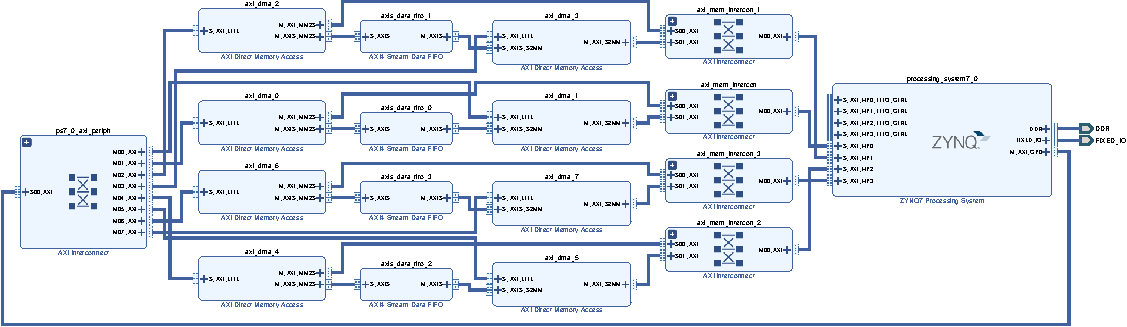
\includegraphics[width=\linewidth]{figures/xilinx_portrait_duplex.pdf}
        \caption{}
        \label{fig:xilinx_duplex}
    \end{subfigure}\\\medskip
    \begin{subfigure}[m]{\linewidth}
        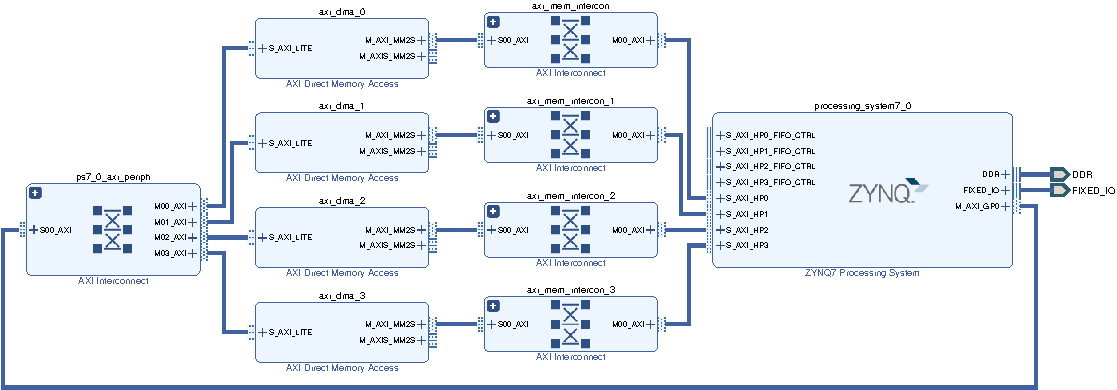
\includegraphics[width=\linewidth]{figures/xilinx_portrait_ps2pl.pdf}
        \caption{}
        \label{fig:xilinx_ps2pl}
    \end{subfigure}\\\medskip
    \begin{subfigure}[m]{\linewidth}
        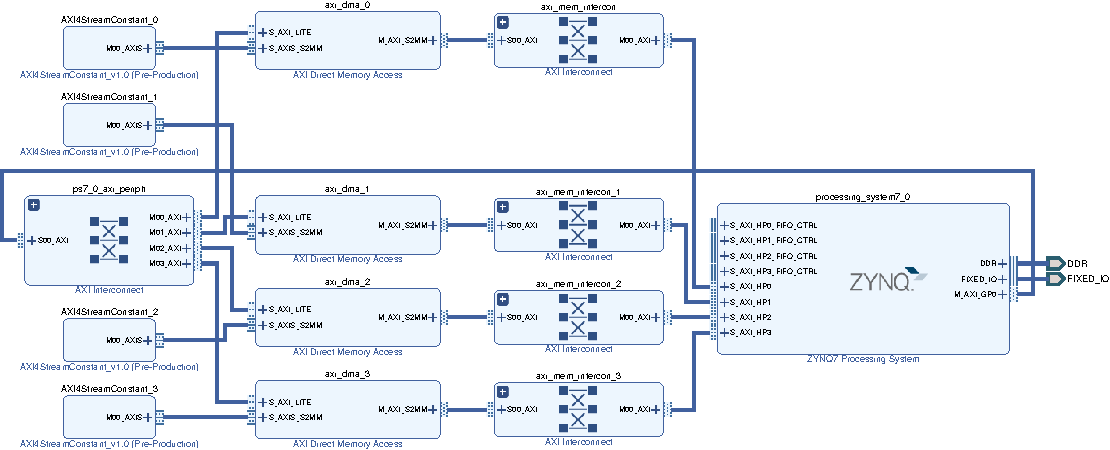
\includegraphics[width=\linewidth]{figures/xilinx_portrait_pl2ps.pdf}
        \caption{}
        \label{fig:xilinx_pl2ps}
    \end{subfigure}
    \caption{Block designs of the systems to evaluate the (\subref{fig:xilinx_duplex}) duplex, (\subref{fig:xilinx_ps2pl}) \ac{PS}-to-\ac{PL}, and (\subref{fig:xilinx_pl2ps}) \ac{PL}-to-\ac{PS} bandwidths of the on-chip high-performance interfaces of the Xilinx device.}
    \label{fig:xilinx_systems}
\end{figure}

To control and monitor the data transfers through the \ac{DMA} engines and calculate their performance, simple bare-metal applications were written using Xilinx hardware libraries and targeted in a single core of the dual-core ARM Cortex-A9 included in the ZYNQ-7010 device.

% TODO bare-metal application

\subsection{Experimental Results}

The three designs were synthesized and implemented using Xilinx Vivado 2018.3 with a \ac{PL} operation frequency of \SI{100}{\mega\hertz}. Additionally, the system depicted in Figure~\ref{fig:xilinx_ps2pl} was also synthesized for an operation frequency of \SI{150}{\mega\hertz}, in an attempt to reproduce the results obtained by G{\"{o}}bel \textit{et al.} regarding the maximum \ac{PS}-to-\ac{PL} bandwidth. All the Xilinx \ac{DMA} devices were configured for a maximum burst size of sixteen, and a maximum stream size of \SI{64}{\mebi\byte}. The four ZYNQ \ac{HP} ports were tested for both 32 and 64-bit configurations. The hardware requirements of the implemented systems are listed in Table~\ref{tab:hardware_xilinx}, in Appendix~\ref{sec:hardware_resources}.

Table \ref{tab:xilinx_results_regular} summarizes the performance results obtained using the three implemented systems. The rows painted in yellow represent configurations in which the bandwidth is degraded compared to the theoretical values. To understand why these configurations lead to sub-optimal bandwidth utilization, the low-level architecture of the ZYNQ-7000 device family has to be considered. As documented in~\cite{xilinx2015zynq}, page 63, the \ac{HP} ports 0 and 1, as well as ports 2 and 3, share the same interconnect to the DDR controller. Naturally, using both \ac{HP} ports 0 and 1 in a 64-bit duplex configuration requires to multiplex a single channel to the DDR controller, leading to a sub-optimal memory bandwidth utilization. However, when using \ac{HP} ports 0 and 2 in the same configuration, two distinct channels to the DDR controller are used, leading to an optimal memory bandwidth utilization close to the maximum theoretical value. It is also worth mentioning the abnormally high standard deviation associated with the sub-optimal configurations, which is most likely due to the entropy generated at the memory controller level. A premise that supports this conclusion is the fact that using \ac{HP} ports 0, 1, and 2 in a 64-bit duplex configuration leads to a lower data rate than using only \ac{HP} ports 0 and 2 in the same configuration.

\begin{figure}[!t]
    \centering
    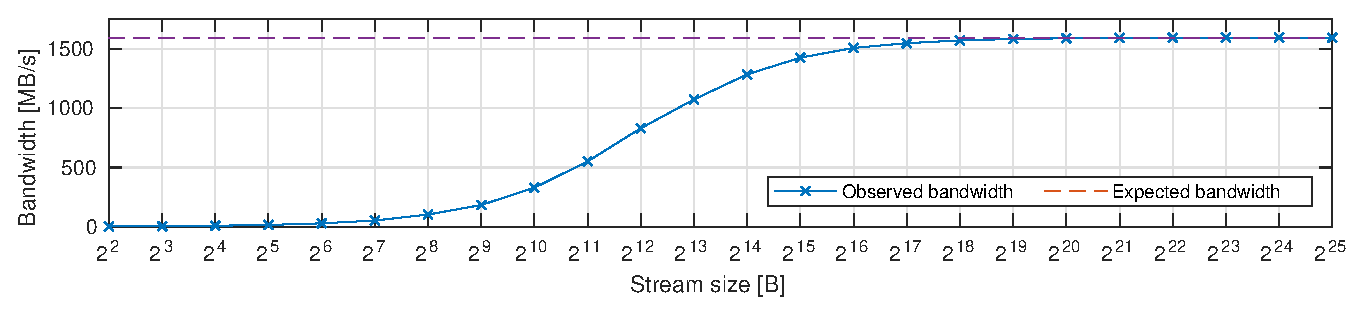
\includegraphics[width=\linewidth]{figures/xilinx_var_stream_size.eps}
    \caption{Observed duplex bandwidth for different stream sizes. The system was designed using a single 64-bit \ac{HP} port and a loop-back \ac{FIFO}, allowing to fully exploit the duplex bandwidth of the \ac{HP} port. The \ac{PL} operation frequency is \SI{100}{\mega\hertz}. Each data point represents the average of 200 transactions of the same size. The maximum standard deviation was \SI{5.70}{\mega\byte\per\second}.}
    \label{fig:xilinx_results_var_size}
\end{figure}

\begin{table}[!b]
\centering
\caption{Expected and observed bandwidth and respective system efficiency for several system configurations using \ac{HP} ports of the ZYNQ-7010 device. Each configuration was tested 200 times for \SI{32}{\mebi\byte} data blocks. The \ac{PL} operating frequency was \SI{100}{\mega\hertz}.}
\label{tab:xilinx_results_regular}
\begin{tabular}{cl|c|r|r|r|r|r|r|}
\cline{3-9}
\multicolumn{1}{l}{}                                                                  &                                                                          &                                            & \multicolumn{5}{c|}{\textbf{Bandwidth [\si{\mega\byte\per\second}]}}                                                                                                                                                      & \multicolumn{1}{c|}{}                                           \\ \cline{4-8}
\multicolumn{1}{l}{}                                                                  &                                                                          &                                            & \multicolumn{1}{c|}{}                                    & \multicolumn{4}{c|}{\textbf{Observed}}                                                                                                                         & \multicolumn{1}{c|}{}                                           \\ \cline{5-8}
\multicolumn{1}{l}{}                                                                  &                                                                          & \multirow{-3}{*}{\textbf{Channels}}        & \multicolumn{1}{c|}{\multirow{-2}{*}{\textbf{Expected}}} & \multicolumn{1}{c|}{\textbf{Average}} & \multicolumn{1}{c|}{\textbf{Minimum}} & \multicolumn{1}{c|}{\textbf{Maximum}} & \multicolumn{1}{c|}{$\mathbf{\sigma}$} & \multicolumn{1}{c|}{\multirow{-3}{*}{\textbf{Efficiency [\%]}}} \\ \hline
\multicolumn{1}{|c|}{}                                                                &                                                                          & \textbf{HP0}                               & 800.00                                                   & 799.95                                & 799.95                                & 799.96                                & 0.0003                                 & 99.99                                                           \\ \cline{3-9} 
\multicolumn{1}{|c|}{}                                                                &                                                                          & \textbf{HP0,1}                             & 1600.00                                                  & 1599.84                               & 1599.84                               & 1599.85                               & 0.0017                                 & 99.99                                                           \\ \cline{3-9} 
\multicolumn{1}{|c|}{}                                                                &                                                                          & \textbf{HP0,2}                             & 1600.00                                                  & 1599.83                               & 1599.79                               & 1599.84                               & 0.0085                                 & 99.99                                                           \\ \cline{3-9} 
\multicolumn{1}{|c|}{}                                                                &                                                                          & \cellcolor[HTML]{FFFF00}\textbf{HP0,1,2}   & \cellcolor[HTML]{FFFF00}2400.00                          & \cellcolor[HTML]{FFFF00}2288.49       & \cellcolor[HTML]{FFFF00}2280.15       & \cellcolor[HTML]{FFFF00}2293.17       & \cellcolor[HTML]{FFFF00}1.2566         & \cellcolor[HTML]{FFFF00}95.35                                   \\ \cline{3-9} 
\multicolumn{1}{|c|}{}                                                                & \multirow{-5}{*}{\textbf{\rotatebox{90}{Duplex}}}                        & \cellcolor[HTML]{FFFF00}\textbf{HP0,1,2,3} & \cellcolor[HTML]{FFFF00}3200.00                          & \cellcolor[HTML]{FFFF00}2773.13       & \cellcolor[HTML]{FFFF00}2697.44       & \cellcolor[HTML]{FFFF00}2789.70       & \cellcolor[HTML]{FFFF00}15.0109        & \cellcolor[HTML]{FFFF00}86.66                                   \\ \cline{2-9} 
\multicolumn{1}{|c|}{}                                                                &                                                                          & \textbf{HP0}                               & 400.00                                                   & 399.99                                & 399.99                                & 399.99                                & 0.0001                                 & 100.00                                                          \\ \cline{3-9} 
\multicolumn{1}{|c|}{}                                                                &                                                                          & \textbf{HP0,1}                             & 800.00                                                   & 799.96                                & 799.96                                & 799.96                                & 0.0006                                 & 100.00                                                          \\ \cline{3-9} 
\multicolumn{1}{|c|}{}                                                                &                                                                          & \textbf{HP0,2}                             & 800.00                                                   & 799.96                                & 799.96                                & 799.96                                & 0.0006                                 & 100.00                                                          \\ \cline{3-9} 
\multicolumn{1}{|c|}{}                                                                &                                                                          & \textbf{HP0,1,2}                           & 1200.00                                                  & 1199.91                               & 1199.91                               & 1199.92                               & 0.0010                                 & 99.99                                                           \\ \cline{3-9} 
\multicolumn{1}{|c|}{}                                                                & \multirow{-5}{*}{\textbf{\rotatebox{90}{PS to PL}}}                      & \textbf{HP0,1,2,3}                         & 1600.00                                                  & 1599.85                               & 1599.85                               & 1599.8521                             & 0.0002                                 & 99.99                                                           \\ \cline{2-9} 
\multicolumn{1}{|c|}{}                                                                &                                                                          & \textbf{HP0}                               & 400.00                                                   & 399.99                                & 399.99                                & 400.0000                              & 0.0078                                 & 100.00                                                          \\ \cline{3-9} 
\multicolumn{1}{|c|}{}                                                                &                                                                          & \textbf{HP0,1}                             & 800.00                                                   & 799.98                                & 799.96                                & 800.0000                              & 0.0229                                 & 100.00                                                          \\ \cline{3-9} 
\multicolumn{1}{|c|}{}                                                                &                                                                          & \textbf{HP0,2}                             & 800.00                                                   & 799.98                                & 799.96                                & 800.0000                              & 0.0228                                 & 100.00                                                          \\ \cline{3-9} 
\multicolumn{1}{|c|}{}                                                                &                                                                          & \textbf{HP0,1,2}                           & 1200.00                                                  & 1199.95                               & 1199.91                               & 1200.0000                             & 0.0493                                 & 100.00                                                          \\ \cline{3-9} 
\multicolumn{1}{|c|}{\multirow{-15}{*}{\textbf{\rotatebox{90}{32 bit per channel}}}} & \multirow{-5}{*}{\textbf{\rotatebox{90}{PL to PS}}}                      & \textbf{HP0,1,2,3}                         & 1600.00                                                  & 1599.92                               & 1599.85                               & 1600.0000                             & 0.0800                                 & 100.00                                                          \\ \hline\hline
\multicolumn{1}{|c|}{}                                                                & \multicolumn{1}{c|}{}                                                    & \textbf{HP0}                               & 1600.00                                                  & 1599.82                               & 1599.81                               & 1599.82                               & 0.0054                                 & 99.99                                                           \\ \cline{3-9} 
\multicolumn{1}{|c|}{}                                                                & \multicolumn{1}{c|}{}                                                    & \cellcolor[HTML]{FFFF00}\textbf{HP0,1}     & \cellcolor[HTML]{FFFF00}3200.00                          & \cellcolor[HTML]{FFFF00}2236.12       & \cellcolor[HTML]{FFFF00}2212.38       & \cellcolor[HTML]{FFFF00}2267.40       & \cellcolor[HTML]{FFFF00}6.3216         & \cellcolor[HTML]{FFFF00}69.88                                   \\ \cline{3-9} 
\multicolumn{1}{|c|}{}                                                                & \multicolumn{1}{c|}{}                                                    & \textbf{HP0,2}                             & 3200.00                                                  & 3197.63                               & 3193.18                               & 3198.68                               & 0.8462                                 & 99.93                                                           \\ \cline{3-9} 
\multicolumn{1}{|c|}{}                                                                & \multicolumn{1}{c|}{}                                                    & \cellcolor[HTML]{FFFF00}\textbf{HP0,1,2}   & \cellcolor[HTML]{FFFF00}4264.00                          & \cellcolor[HTML]{FFFF00}2659.35       & \cellcolor[HTML]{FFFF00}2639.86       & \cellcolor[HTML]{FFFF00}2682.41       & \cellcolor[HTML]{FFFF00}4.1705         & \cellcolor[HTML]{FFFF00}62.37                                   \\ \cline{3-9} 
\multicolumn{1}{|c|}{}                                                                & \multicolumn{1}{c|}{\multirow{-5}{*}{\textbf{\rotatebox{90}{Duplex}}}}   & \cellcolor[HTML]{FFFF00}\textbf{HP0,1,2,3} & \cellcolor[HTML]{FFFF00}4264.00                          & \cellcolor[HTML]{FFFF00}2675.65       & \cellcolor[HTML]{FFFF00}2108.10       & \cellcolor[HTML]{FFFF00}2969.61       & \cellcolor[HTML]{FFFF00}297.1049       & \cellcolor[HTML]{FFFF00}62.75                                   \\ \cline{2-9} 
\multicolumn{1}{|c|}{}                                                                & \multicolumn{1}{c|}{}                                                    & \textbf{HP0}                               & 800.00                                                   & 799.96                                & 799.95                                & 799.96                                & 0.0012                                 & 99.99                                                           \\ \cline{3-9} 
\multicolumn{1}{|c|}{}                                                                & \multicolumn{1}{c|}{}                                                    & \textbf{HP0,1}                             & 1600.00                                                  & 1599.84                               & 1599.83                               & 1599.84                               & 0.0018                                 & 99.99                                                           \\ \cline{3-9} 
\multicolumn{1}{|c|}{}                                                                & \multicolumn{1}{c|}{}                                                    & \textbf{HP0,2}                             & 1600.00                                                  & 1599.84                               & 1599.83                               & 1599.85                               & 0.0016                                 & 99.99                                                           \\ \cline{3-9} 
\multicolumn{1}{|c|}{}                                                                & \multicolumn{1}{c|}{}                                                    & \textbf{HP0,1,2}                           & 2400.00                                                  & 2399.66                               & 2399.64                               & 2399.66                               & 0.0054                                 & 99.99                                                           \\ \cline{3-9} 
\multicolumn{1}{|c|}{}                                                                & \multicolumn{1}{c|}{\multirow{-5}{*}{\textbf{\rotatebox{90}{PS to PL}}}} & \textbf{HP0,1,2,3}                         & 3200.00                                                  & 3184.87                               & 3103.57                               & 3199.38                               & 16.7246                                & 99.53                                                           \\ \cline{2-9} 
\multicolumn{1}{|c|}{}                                                                & \multicolumn{1}{c|}{}                                                    & \textbf{HP0}                               & 800.00                                                   & 799.98                                & 799.95                                & 800.00                                & 0.0286                                 & 100.00                                                          \\ \cline{3-9} 
\multicolumn{1}{|c|}{}                                                                & \multicolumn{1}{c|}{}                                                    & \textbf{HP0,1}                             & 1600.00                                                  & 1599.91                               & 1599.83                               & 1600.00                               & 0.0917                                 & 99.99                                                           \\ \cline{3-9} 
\multicolumn{1}{|c|}{}                                                                & \multicolumn{1}{c|}{}                                                    & \textbf{HP0,2}                             & 1600.00                                                  & 1599.91                               & 1599.83                               & 1600.00                               & 0.0914                                 & 100.00                                                          \\ \cline{3-9} 
\multicolumn{1}{|c|}{}                                                                & \multicolumn{1}{c|}{}                                                    & \textbf{HP0,1,2}                           & 2400.00                                                  & 2399.83                               & 2399.63                               & 2400.00                               & 0.1895                                 & 99.99                                                           \\ \cline{3-9} 
\multicolumn{1}{|c|}{\multirow{-15}{*}{\textbf{\rotatebox{90}{64 bit per channel}}}} & \multicolumn{1}{c|}{\multirow{-5}{*}{\textbf{\rotatebox{90}{PL to PS}}}} & \textbf{HP0,1,2,3}                         & 3200.00                                                  & 3199.70                               & 3199.39                               & 3200.00                               & 0.3170                                 & 99.99                                                           \\ \hline
\end{tabular}
\end{table} %

Although the previous experiments allowed to fully exploit the bandwidth of the on-chip high-performance interfaces in duplex mode, they were insufficient to reproduce the results obtained by G{\"{o}}bel \textit{et al.} regarding the \ac{PS}-to-\ac{PL} bandwidth of the Xilinx device. In order to increase even further the bandwidth requirement on the \ac{PL} side, the system to evaluate the \ac{PS}-to-\ac{PL} bandwidth was re-implemented for an operating frequency of \SI{150}{\mega\hertz}. With the new operation frequency, the \ac{PL} component of the system is capable of a maximum data rate of \SI{4800}{\mega\byte\per\second}, which is even higher than the DDR maximum bandwidth. The results of this experiment are shown in Table \ref{tab:results_xilinx_stress_150}. As expected, the maximum achieved bandwidth surpasses that of the same system implemented for an operating frequency of \SI{100}{MHz}. The configuration that leads, in average, to the highest data rate (\SI{3448.33}{\mega\byte\per\second}) is the one using \ac{HP} ports 0, 1 and 2. The maximum achieved data rate is compatible with the conclusions of G{\"{o}}bel \textit{et al.} Furthermore, in one or more experiments using all the four \ac{HP} ports, a bandwidth higher than \SI{4}{\giga\byte\per\second} was obtained. However, such performance is not always possible due to limitations at the memory controller level. It is also worth mentioning that, under stress, the \ac{HP} ports achieve higher data rates on single-sided transfers than on duplex transfers.

\begin{table}[!b]
\centering
\caption{Expected and observed bandwidth and respective system efficiency for configurations aiming at exploiting the maximum \ac{PS}-to-\ac{PL} bandwidth. Each configuration was tested 200 times for \SI{32}{\mebi\byte} data blocks. The \ac{PL} operating frequency was \SI{150}{\mega\hertz}.}
\label{tab:results_xilinx_stress_150}
\begin{tabular}{c|c|r|r|r|r|r|r|}
\cline{2-8}
                                                                                                                    &                                            & \multicolumn{5}{c|}{\textbf{Bandwidth [\si{\mega\byte\per\second}]}}                                                                                                                                                      & \multicolumn{1}{c|}{}                                           \\ \cline{3-7}
                                                                                                                    &                                            & \multicolumn{1}{c|}{}                                    & \multicolumn{4}{c|}{\textbf{Observed}}                                                                                                                         & \multicolumn{1}{c|}{}                                           \\ \cline{4-7}
                                                                                                                    & \multirow{-3}{*}{\textbf{Channels}}        & \multicolumn{1}{c|}{\multirow{-2}{*}{\textbf{Expected}}} & \multicolumn{1}{c|}{\textbf{Average}} & \multicolumn{1}{c|}{\textbf{Minimum}} & \multicolumn{1}{c|}{\textbf{Maximum}} & \multicolumn{1}{c|}{$\mathbf{\sigma}$} & \multicolumn{1}{c|}{\multirow{-3}{*}{\textbf{Efficiency [\%]}}} \\ \hline
\multicolumn{1}{|c|}{}                                                                                              & \textbf{HP0}                               & 1200                                                     & 1199.91                               & 1199.91                               & 1199.91                               & 0.0005                                 & 99.99                                                           \\ \cline{2-8} 
\multicolumn{1}{|c|}{}                                                                                              & \textbf{HP0,1}                             & 2400                                                     & 2393.39                               & 2371.02                               & 2397.02                               & 2.3698                                 & 99.72                                                           \\ \cline{2-8} 
\multicolumn{1}{|c|}{}                                                                                              & \textbf{HP0,2}                             & 2400                                                     & 2396.52                               & 2396.07                               & 2398.13                               & 0.2730                                 & 99.86                                                           \\ \cline{2-8} 
\multicolumn{1}{|c|}{}                                                                                              & \cellcolor[HTML]{FFFF00}\textbf{HP0,1,2}   & \cellcolor[HTML]{FFFF00}3600                             & \cellcolor[HTML]{FFFF00}3448.33       & \cellcolor[HTML]{FFFF00}3413.08       & \cellcolor[HTML]{FFFF00}3510.90       & \cellcolor[HTML]{FFFF00}11.2324        & \cellcolor[HTML]{FFFF00}95.79                                   \\ \cline{2-8} 
\multicolumn{1}{|c|}{\multirow{-5}{*}{\textbf{\begin{tabular}[c]{@{}c@{}}64 bit/\\ channel,\\ PS to PL\end{tabular}}}} & \cellcolor[HTML]{FFFF00}\textbf{HP0,1,2,3} & \cellcolor[HTML]{FFFF00}4264                             & \cellcolor[HTML]{FFFF00}3154.97       & \cellcolor[HTML]{FFFF00}2939.33       & \cellcolor[HTML]{FFFF00}4001.69       & \cellcolor[HTML]{FFFF00}133.1674       & \cellcolor[HTML]{FFFF00}73.99                                   \\ \hline
\end{tabular}
\end{table} %

To conclude the assessment of the ZYNQ-7000 device, another scenario based on the system to evaluate the duplex bandwidth was considered in which streams of multiple sizes were transferred from the \ac{PS} to the \ac{PL} and back to the \ac{PS}. For this experiment, a single 64-bit \ac{HP} port was used, the \ac{PL} operation frequency was set to \SI{100}{\mega\hertz}, and each stream size was tested 200 times. Figure \ref{fig:xilinx_results_var_size} illustrates the results of this experiment. Results show that small stream sizes only achieve a fraction of the theoretical maximum bandwidth allowed by the used configuration. Only for streams bigger than \SI{64}{\kibi\byte} a real bandwidth of more than 90\% of the theoretical maximum is achieved.

%\clearpage %
\section{Intel Cyclone V SE device}\label{sec:intel}

Similarly to the assessment of the ZYNQ-7010 device, the same three systems depicted in Figure~\ref{fig:evaluation_circuit} were implemented and targeted in the Cyclone V SE device. Since the Cyclone V device family only has one on-chip high-performance port that connects the \ac{FPGA} to the DDR controller through the \ac{HPS}, a single \ac{DMA} engine was used in each system. The used \ac{DMA} engine was Intel's \ac{MSGDMA}, which revealed capable of fully-exploiting the bandwidth of the \ac{F2S} interface. The Intel's \ac{MSGDMA} allows three configurations regarding its input and output interfaces: AXI3-to-AXI3, AXI3-to-Avalon-Stream, and Avalon-Stream-to-AXI3. Furthermore, the \ac{MSGDMA} also includes an internal data \ac{FIFO}, which allows simplifying the system to assess the duplex bandwidth by using the \ac{MSGDMA} in the configuration AXI3-to-AXI3 and connecting both interfaces to the \ac{F2S} port directly, as shown in Figure~\ref{fig:intel_duplex}. Note that both the AXI3 interfaces of the \ac{MSGDMA} can be connected to the \ac{F2S} port even if they have \SI{256}{\bit} each. This is only possible because each of these interfaces is single-sided (one interface only reads and the other only writes), and the \ac{F2S} port is full-duplex. For testing the \ac{HPS}-to-\ac{FPGA} and the \ac{FPGA}-to-\ac{HPS} bandwidths, the \ac{MSGDMA} was configured as AXI3-to-Avalon-Stream and Avalon-Stream-to-AXI3, respectively. Additionally, two simple circuits were developed to absorb the stream generated by the \ac{MSGDMA} in the configuration AXI3-to-Avalon-Stream and generate a data stream to be absorbed by the \ac{MSGDMA} in the configuration Avalon-Stream-to-AXI3. In resemblance to the system targeting the Xilinx device, the circuit to absorb the stream consists of a single wire connected to the \textit{ready} signal of the Avalon-Stream master interface. On the other hand, the circuit to produce a data stream to be transmitted to the \ac{MSGDMA} engine is simpler than its Xilinx counterpart. The streaming protocol used by the Xilinx \ac{DMA} device is the AXI4-Stream protocol, which features signal indicating the end of the stream. Therefore, a \ac{FSM} is needed to count the elements of the stream and activate the \textit{last} signal during the transmission of the stream's last element. However, the streaming protocol used by Intel's \ac{MSGDMA} (Avalon-Stream~\cite{intel2020avalon}) does not have a signal indicating the end of the stream. Thus, there is no need for a \ac{FSM}. To produce a constant stream, it only takes to set the \textit{data} bus to a constant and the \textit{valid} signal to high. Figures~\ref{fig:intel_h2f} and \ref{fig:intel_f2h} illustrate the systems to evaluate the \ac{HPS}-to-\ac{FPGA} and \ac{FPGA}-to-\ac{HPS} bandwidths, respectively.

\begin{figure}[!b]
    \centering
    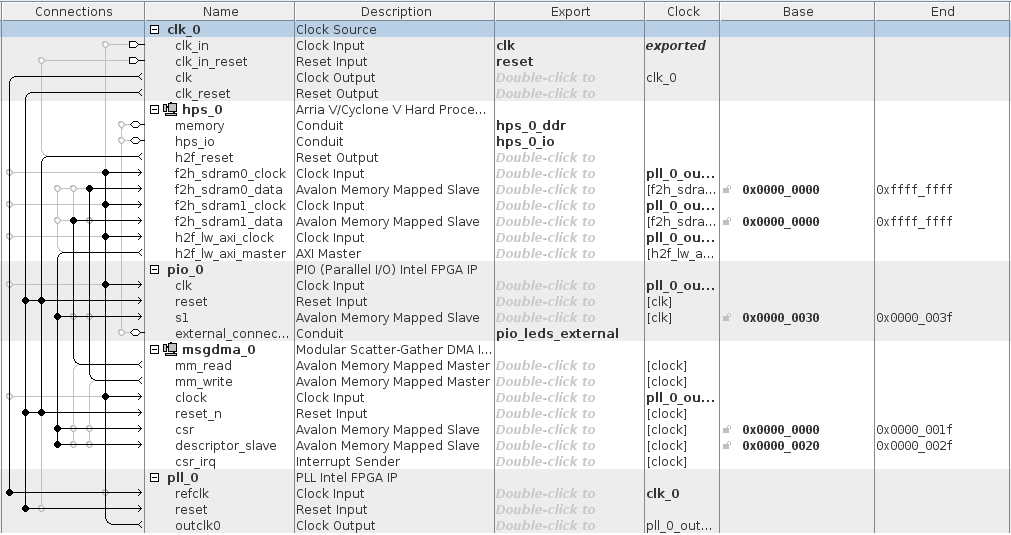
\includegraphics[width=\linewidth]{figures/intel_duplex.png}
    \caption{Schematic of the system to assess the duplex bandwidth of the on-chip high-performance interfaces of the Intel device, as shown in the Platform Designer tool of Intel Quartus Prime.}
    \label{fig:intel_duplex}
\end{figure}

\begin{figure}[!t]
    \centering
    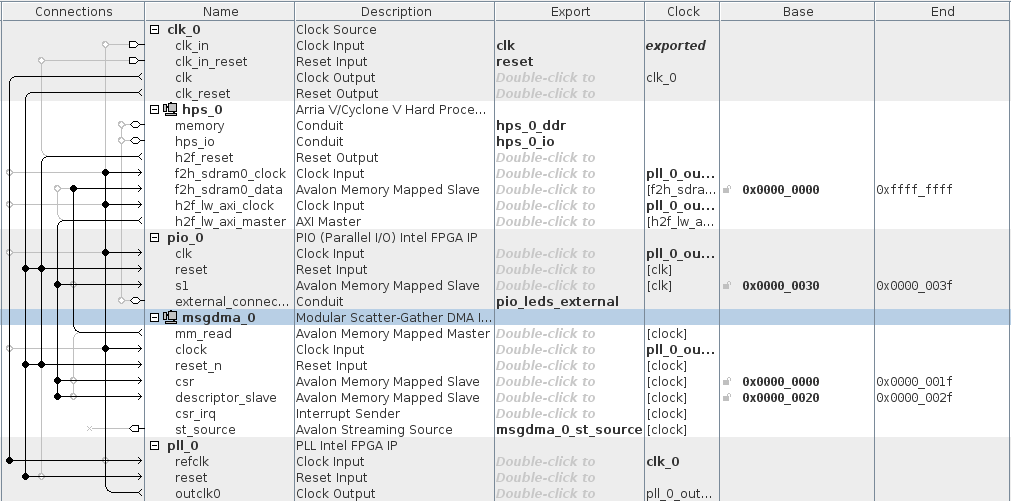
\includegraphics[width=\linewidth]{figures/intel_h2f.png}
    \caption{Schematic of the system to assess the \ac{HPS}-to-\ac{FPGA} bandwidth of the on-chip high-performance interfaces of the Intel device, as shown in the Platform Designer tool of Intel Quartus Prime.}
    \label{fig:intel_h2f}
\end{figure}

\begin{figure}[!t]
    \centering
    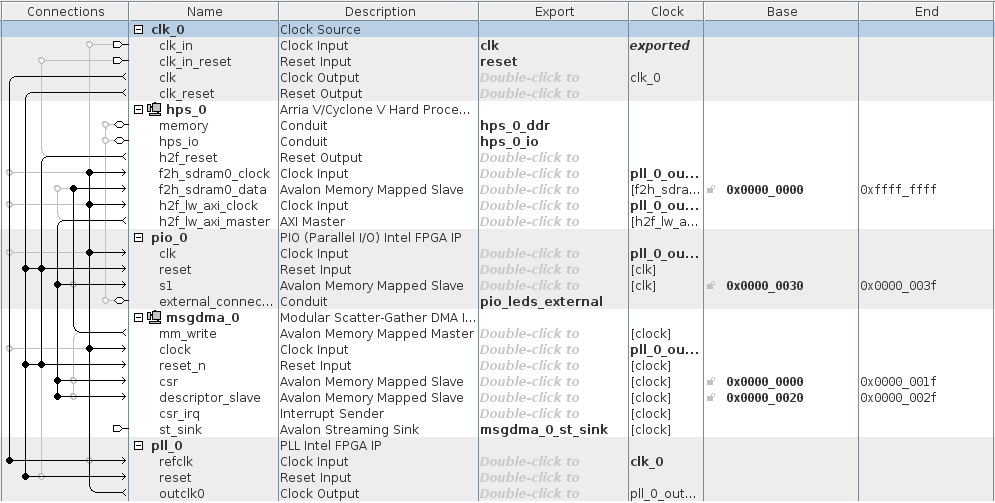
\includegraphics[width=\linewidth]{figures/intel_f2h.png}
    \caption{Schematic of the system to assess the \ac{FPGA}-to-\ac{HPS} bandwidth of the on-chip high-performance interfaces of the Intel device, as shown in the Platform Designer tool of Intel Quartus Prime.}
    \label{fig:intel_f2h}
\end{figure}

In contrast with the software framework for controlling and monitoring the \ac{FPGA}-implemented circuits in the Xilinx device (which was bare-metal), the software used to control the \ac{FPGA} components on the Intel device was developed to be executed in Linux environment. This implementation choice had to do with the poorer bare-metal development support provided by Intel tools when comparing to Xilinx's more powerful and automated tools. For instance, compiling a bare-metal application for Intel devices requires the developer to write a linker script by hand (there is no tool to generate the linker script automatically). Although Intel provides linker scripts that can be used out-of-the-box, they only work for certain applications. Another possibility is to use the ARM compiler, instead of the default Intel bare-metal compiler, which requires the user to write a scatter file. Although scatter files are usually much less verbose than linker scripts, their syntax is also complex. Naturally, the examples of scatter files provided by ARM also have a limited scope. In contrast with bare-metal, Linux development is much more powerful and there are simple known techniques to overcome issues such as addressing memory-mapped peripherals through their physical addresses, or reserve part of the DDR memory to be used directly by \ac{DMA} engines without needing to translate virtual addresses. As explained by Kashani \textit{et al.}~\cite{sahandSoCTutorial}, the physical addresses of the memory-mapped peripherals can be accessed from the Linux system using the function \texttt{mmap} to map those addresses into addresses in the application addressing space. To reserve part of the DDR to be used directly by \ac{DMA} engines, it is possible to assign only a sub-region of the DDR to the Linux kernel at boot time, leaving the upper addresses free. By default, the upper part of the DDR that is not used by the Linux kernel is ignored by the operating system and is initialized as non-cacheable memory. However, it can still be accessed using the same method to address the memory-mapped peripherals, using the \texttt{mmap} function to map the physical addresses of the upper DDR region into addresses in the application addressing space.

\subsection{Experimental Results}

The three systems to evaluate the bandwidth of the on-chip high-performance interfaces of the Cyclone V device were implemented using Intel Quartus Prime 18.1 with a \ac{FPGA} operation frequency of \SI{100}{\mega\hertz}. The \ac{MSGDMA} was configured for a maximum burst size of sixteen, and a maximum stream size of \SI{256}{\mega\byte}. The \ac{F2S} port was tested for 32, 64, 128 and 256-bit configurations. The hardware requirements of the implemented systems are listed in Table~\ref{tab:hardware_intel}, in Appendix~\ref{sec:hardware_resources}.

Table \ref{tab:intel_results_regular} summarizes the performance results obtained using all the three systems. The rows painted in yellow correspond to sub-optimal configurations whose bandwidth is degraded compared with the theoretically expected. The highest bandwidth (\SI{2779.05}{\mega\byte\per\second}) was achieved for \ac{HPS}-to-\ac{FPGA} transfers using all the \SI{256}{bit} of the \ac{F2S} port, which is compatible with the results obtained by G{\"{o}}bel \textit{et al.}. Similarly to the Xilinx device, for configurations where the \ac{F2S} interface is wider, the bandwidth is degraded. Furthermore, that effect is exaggerated by the lower operating frequency of the DRAM connected to the Cyclone V device comparing with the one connected to the ZYNQ-7000 device, which leads to a lower DRAM bandwidth. It is also worth noticing that the maximum bandwidth allowed for duplex transfers is lower than the one associated with single-sided transfers. This effect is also visible in the results regarding the Xilinx device and can be attributed to the entropy generated at the DRAM controller level when multiplexing the DDR ports to read and write data at data rates close to the DRAM's limit. This hypothesis is supported by the higher standard deviations associated with the results of experiments using those configurations, which indicate that they are not completely deterministic.

\begin{table}[!b]
\centering
\caption{Expected and observed bandwidth and respective system efficiency for several system configurations using \ac{F2S} ports of the Cyclone V device. Each configuration was tested 200 times for \SI{32}{\mebi\byte} data blocks. The \ac{FPGA} operating frequency was \SI{100}{\mega\hertz}. Note that H2F stands for \ac{HPS}-to-\ac{FPGA}, and F2H means \ac{FPGA}-to-\ac{HPS}.}
\label{tab:intel_results_regular}
\begin{tabular}{l|c|r|r|r|r|r|r|}
\cline{2-8}
                                                                        &                                                                                                & \multicolumn{5}{c|}{\textbf{Bandwidth [\si{\mega\byte\per\second}]}}                                                                                                                                                      & \multicolumn{1}{c|}{}                                           \\ \cline{3-7}
                                                                        &                                                                                                & \multicolumn{1}{c|}{}                                    & \multicolumn{4}{c|}{\textbf{Observed}}                                                                                                                         & \multicolumn{1}{c|}{}                                           \\ \cline{4-7}
                                                                        & \multirow{-3}{*}{\textbf{\begin{tabular}[c]{@{}c@{}}Channel\\ Width [\si{\bit}]\end{tabular}}} & \multicolumn{1}{c|}{\multirow{-2}{*}{\textbf{Expected}}} & \multicolumn{1}{c|}{\textbf{Average}} & \multicolumn{1}{c|}{\textbf{Minimum}} & \multicolumn{1}{c|}{\textbf{Maximum}} & \multicolumn{1}{c|}{$\mathbf{\sigma}$} & \multicolumn{1}{c|}{\multirow{-3}{*}{\textbf{Efficiency [\%]}}} \\ \hline
\multicolumn{1}{|l|}{}                                                  & \textbf{32}                                                                                    & 800.00                                                   & 799.59                                & 799.04                                & 799.91                                & 0.1279                                 & 99.95                                                           \\ \cline{2-8} 
\multicolumn{1}{|l|}{}                                                  & \textbf{64}                                                                                    & 1600.00                                                  & 1579.80                               & 1563.76                               & 1583.54                               & 3.1448                                 & 98.74                                                           \\ \cline{2-8} 
\multicolumn{1}{|l|}{}                                                  & \cellcolor[HTML]{FFFF00}\textbf{128}                                                           & \cellcolor[HTML]{FFFF00}3200.00                          & \cellcolor[HTML]{FFFF00}2019.26       & \cellcolor[HTML]{FFFF00}1836.18       & \cellcolor[HTML]{FFFF00}2023.30       & \cellcolor[HTML]{FFFF00}13.9767        & \cellcolor[HTML]{FFFF00}63.10                                   \\ \cline{2-8} 
\multicolumn{1}{|l|}{\multirow{-4}{*}{\textbf{\rotatebox{90}{Duplex}}}} & \cellcolor[HTML]{FFFF00}\textbf{256}                                                           & \cellcolor[HTML]{FFFF00}3200.00                          & \cellcolor[HTML]{FFFF00}2037.16       & \cellcolor[HTML]{FFFF00}1885.93       & \cellcolor[HTML]{FFFF00}2039.91       & \cellcolor[HTML]{FFFF00}13.1620        & \cellcolor[HTML]{FFFF00}63.66                                   \\ \hline
\multicolumn{1}{|l|}{}                                                  & \textbf{32}                                                                                    & 400.00                                                   & 399.81                                & 399.69                                & 399.96                                & 0.0299                                 & 99.95                                                           \\ \cline{2-8} 
\multicolumn{1}{|l|}{}                                                  & \textbf{64}                                                                                    & 800.00                                                   & 799.60                                & 797.81                                & 799.87                                & 0.1862                                 & 99.95                                                           \\ \cline{2-8} 
\multicolumn{1}{|l|}{}                                                  & \textbf{128}                                                                                   & 1600.00                                                  & 1569.88                               & 1561.47                               & 1570.90                               & 1.5062                                 & 98.12                                                           \\ \cline{2-8} 
\multicolumn{1}{|l|}{\multirow{-4}{*}{\textbf{\rotatebox{90}{H2F}}}}    & \cellcolor[HTML]{FFFF00}\textbf{256}                                                           & \cellcolor[HTML]{FFFF00}3200.00                          & \cellcolor[HTML]{FFFF00}2779.05       & \cellcolor[HTML]{FFFF00}2736.46       & \cellcolor[HTML]{FFFF00}2790.85       & \cellcolor[HTML]{FFFF00}5.9443         & \cellcolor[HTML]{FFFF00}86.85                                   \\ \hline
\multicolumn{1}{|l|}{}                                                  & \textbf{32}                                                                                    & 400.00                                                   & 399.81                                & 399.70                                & 399.95                                & 0.0333                                 & 99.95                                                           \\ \cline{2-8} 
\multicolumn{1}{|l|}{}                                                  & \textbf{64}                                                                                    & 800.00                                                   & 799.59                                & 797.83                                & 799.87                                & 0.2206                                 & 99.95                                                           \\ \cline{2-8} 
\multicolumn{1}{|l|}{}                                                  & \textbf{128}                                                                                   & 1600.00                                                  & 1576.78                               & 1574.66                               & 1579.18                               & 1.8717                                 & 98.55                                                           \\ \cline{2-8} 
\multicolumn{1}{|l|}{\multirow{-4}{*}{\textbf{\rotatebox{90}{F2H}}}}    & \cellcolor[HTML]{FFFF00}\textbf{256}                                                           & \cellcolor[HTML]{FFFF00}3200.00                          & \cellcolor[HTML]{FFFF00}2464.66       & \cellcolor[HTML]{FFFF00}2137.91       & \cellcolor[HTML]{FFFF00}2473.06       & \cellcolor[HTML]{FFFF00}32.3298        & \cellcolor[HTML]{FFFF00}77.02                                   \\ \hline
\end{tabular}
\end{table} %

Concluding the analysis of the Cyclone V device family, a final scenario based on the system to evaluate the duplex bandwidth was considered. The \ac{F2S} port was configured to use only \SI{64}{bit} and the system was implemented targeting an operation frequency of \SI{100}{\mega\hertz}. This experiment consisted of transferring streams of multiple sizes from the \ac{HPS} to the \ac{FPGA} and back to the \ac{HPS}. Each stream size was tested 200 times, and the results were averaged. Figure \ref{fig:intel_results_var_size} illustrates the results of this experiment. Results show that small stream sizes only achieve a fraction of the theoretical maximum bandwidth allowed by the \ac{F2S} port. Only for stream sizes bigger than \SI{512}{\kibi\byte} a real bandwidth of more than 90\% of the theoretical maximum is achieved.

\begin{figure}[t]
    \centering
    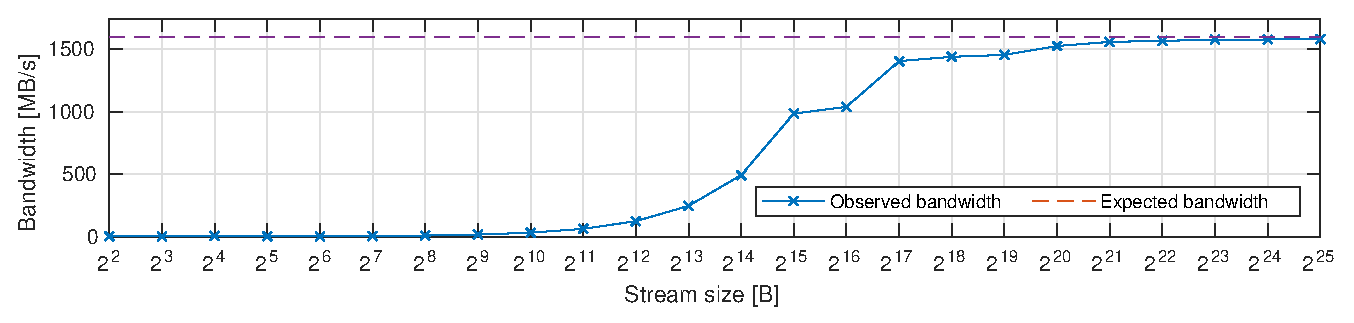
\includegraphics[width=\linewidth]{figures/intel_var_stream_size.eps}
    \caption{Observed duplex bandwidth for different stream sizes. The system was designed using a 64-bit \ac{F2S} port and a loop-back \ac{FIFO}, allowing to fully exploit the duplex bandwidth of the \ac{F2S} port. The \ac{FPGA} operation frequency is \SI{100}{\mega\hertz}. Each data point represents the average of 200 transactions of the same size. The maximum standard deviation was \SI{42.19}{\mega\byte\per\second}.}
    \label{fig:intel_results_var_size}
\end{figure} %
\section{Conclusions}\label{sec:conclusions}

This work aimed at evaluating the performance of the on-chip high-performance interfaces of Xilinx and Intel's low-end \ac{FPGA}-\ac{SoC} device families (ZYNQ-7000 and Cyclone V, respectively). For achieving that goal, three systems were designed to fully exploit the duplex, \ac{PS}-to-\ac{PL}, and \ac{PL}-to-\ac{PS} bandwidths. Then, those systems were implemented and targeted on both Xilinx ZYNQ-7010 and Intel Cyclone V SE devices. Multiple implementation options were considered regarding the choice of \ac{DMA} engines to use on each device and the software environment running on the hard \acp{CPU} of the \ac{FPGA}-\acp{SoC} (bare-metal or Linux).

The obtained results were compared to the results obtained by G{\"{o}}bel \textit{et al.} in a previous study, and also with the theoretical limits of the devices. The maximum observed data rates are similar to the ones observed by G{\"{o}}bel \textit{et al.} Additionally, the results suggest that the bandwidth allowed by the on-chip high-performance channels of both devices is limited by the memory controller. Whenever getting close to the DDR maximum data rate, the bandwidth starts to degrade. Furthermore, the higher bandwidths achieved by single-sided transfers and the higher standard deviations associated with experiments using sub-optimal configurations suggest that there is some level of entropy at the memory controller level that affects the performance negatively.

The artifact produced by this work and its support documentation can be found at \url{https://github.com/joaomiguelvieira/FPGA_SoC_DMA_stress/}. %
\section*{Acknowledgments}

I would like to thank Professor Horácio Neto and Professor Rui Duarte for their support and guidance during the execution of this project.

I also thank Sahand Kashani for his support, namely the numerous hours spent on debugging the designs for the Intel \ac{FPGA}-\ac{SoC} device.
 %
%
\bibliographystyle{unsrt} %
\bibliography{bibliography} %
%
\appendix %
\section{Hardware Resources}\label{sec:hardware_resources} %
%
\begin{table}[htb]
\centering
\caption{Hardware requirements of the systems to assess the on-chip high-performance interfaces of the Xilinx ZYNQ-7010 device.}
\label{tab:hardware_xilinx}
\begin{tabular}{c|c|rr|rr|rr|rr|}
\cline{2-10}
\multicolumn{1}{l|}{}                                                 &                                                                                                & \multicolumn{8}{c|}{\textbf{Hardware Resources}}                                                                                                                                                    \\ \cline{3-10} 
\multicolumn{1}{l|}{}                                                 & \multirow{-2}{*}{\textbf{\begin{tabular}[c]{@{}c@{}}Channel Width\\{} [bit/channel]\end{tabular}}} & \multicolumn{2}{c|}{\textbf{\acsp{LUT} (17600)}} & \multicolumn{2}{c|}{\textbf{\acsp{FF} (35200)}} & \multicolumn{2}{c|}{\textbf{\acsp{BRAM} (60)}} & \multicolumn{2}{c|}{\textbf{\acsp{DSP} (80)}} \\ \hline
\multicolumn{1}{|c|}{}                                                & \textbf{32}                                                                                    & 8581     & \cellcolor[HTML]{C0C0C0}(48.76 \%)    & 11702    & \cellcolor[HTML]{C0C0C0}(33.24 \%)   & 14     & \cellcolor[HTML]{C0C0C0}(23.33 \%)    & 0     & \cellcolor[HTML]{C0C0C0}(0.00 \%)     \\ \cline{2-10} 
\multicolumn{1}{|c|}{\multirow{-2}{*}{\textbf{Duplex}}}               & \textbf{64}                                                                                    & 10045    & \cellcolor[HTML]{C0C0C0}(57.07 \%)    & 13594    & \cellcolor[HTML]{C0C0C0}(38.62 \%)   & 22     & \cellcolor[HTML]{C0C0C0}(36.67 \%)    & 0     & \cellcolor[HTML]{C0C0C0}(0.00 \%)     \\ \hline
\multicolumn{1}{|c|}{}                                                & \textbf{32}                                                                                    & 2623     & \cellcolor[HTML]{C0C0C0}(14.90 \%)    & 3769     & \cellcolor[HTML]{C0C0C0}(10.71 \%)   & 4      & \cellcolor[HTML]{C0C0C0}(6.67 \%)     & 0     & \cellcolor[HTML]{C0C0C0}(0.00 \%)     \\ \cline{2-10} 
\multicolumn{1}{|c|}{\multirow{-2}{*}{\textbf{\acs{PS} to \acs{PL}}}} & \textbf{64}                                                                                    & 2656     & \cellcolor[HTML]{C0C0C0}(15.09 \%)    & 3697     & \cellcolor[HTML]{C0C0C0}(10.50 \%)   & 2      & \cellcolor[HTML]{C0C0C0}(3.33 \%)     & 0     & \cellcolor[HTML]{C0C0C0}(0.00 \%)     \\ \hline
\multicolumn{1}{|c|}{}                                                & \textbf{32}                                                                                    & 5060     & \cellcolor[HTML]{C0C0C0}(28.75 \%)    & 6685     & \cellcolor[HTML]{C0C0C0}(18.99 \%)   & 4      & \cellcolor[HTML]{C0C0C0}(6.67 \%)     & 0     & \cellcolor[HTML]{C0C0C0}(0.00 \%)     \\ \cline{2-10} 
\multicolumn{1}{|c|}{\multirow{-2}{*}{\textbf{\acs{PL} to \acs{PS}}}} & \textbf{64}                                                                                    & 5671     & \cellcolor[HTML]{C0C0C0}(32.22 \%)    & 7421     & \cellcolor[HTML]{C0C0C0}(21.08 \%)   & 6      & \cellcolor[HTML]{C0C0C0}(10.00 \%)    & 0     & \cellcolor[HTML]{C0C0C0}(0.00 \%)     \\ \hline
\end{tabular}
\end{table} %
\begin{table}[htb]
\centering
\caption{Hardware requirements of the systems to assess the on-chip high-performance interfaces of the Intel Cyclone V SE device.}
\label{tab:hardware_intel}
\begin{tabular}{c|c|rr|r|rr|rr|}
\cline{2-9}
\multicolumn{1}{l|}{}                                                    &                                                                                                & \multicolumn{7}{c|}{\textbf{Hardware Resources}}                                                                                                                          \\ \cline{3-9} 
\multicolumn{1}{l|}{}                                                    & \multirow{-2}{*}{\textbf{\begin{tabular}[c]{@{}c@{}}Channel\\ Width [\si{\bit}]\end{tabular}}} & \multicolumn{2}{c|}{\textbf{\acsp{ALM}}} & \multicolumn{1}{c|}{\textbf{Registers}} & \multicolumn{2}{c|}{\textbf{\acsp{BRAM}}} & \multicolumn{2}{c|}{\textbf{\acsp{DSP}}} \\ \hline
\multicolumn{1}{|c|}{}                                                   & \textbf{32}                                                                                    & 1036 & \cellcolor[HTML]{C0C0C0}(3.23 \%) & 1538                                    & 14  & \cellcolor[HTML]{C0C0C0}(3.53 \%)   & 0   & \cellcolor[HTML]{C0C0C0}(0.00 \%)  \\ \cline{2-9} 
\multicolumn{1}{|c|}{}                                                   & \textbf{64}                                                                                    & 1033 & \cellcolor[HTML]{C0C0C0}(3.22 \%) & 1536                                    & 20  & \cellcolor[HTML]{C0C0C0}(5.04 \%)   & 0   & \cellcolor[HTML]{C0C0C0}(0.00 \%)  \\ \cline{2-9} 
\multicolumn{1}{|c|}{}                                                   & \textbf{128}                                                                                   & 1064 & \cellcolor[HTML]{C0C0C0}(3.32 \%) & 1537                                    & 32  & \cellcolor[HTML]{C0C0C0}(8.06 \%)   & 0   & \cellcolor[HTML]{C0C0C0}(0.00 \%)  \\ \cline{2-9} 
\multicolumn{1}{|c|}{\multirow{-4}{*}{\textbf{Duplex}}}                  & \textbf{256}                                                                                   & 1105 & \cellcolor[HTML]{C0C0C0}(3.45 \%) & 1535                                    & 58  & \cellcolor[HTML]{C0C0C0}(14.61 \%)  & 0   & \cellcolor[HTML]{C0C0C0}(0.00 \%)  \\ \hline
\multicolumn{1}{|c|}{}                                                   & \textbf{32}                                                                                    & 803  & \cellcolor[HTML]{C0C0C0}(2.50 \%) & 1270                                    & 3   & \cellcolor[HTML]{C0C0C0}(0.76 \%)   & 0   & \cellcolor[HTML]{C0C0C0}(0.00 \%)  \\ \cline{2-9} 
\multicolumn{1}{|c|}{}                                                   & \textbf{64}                                                                                    & 817  & \cellcolor[HTML]{C0C0C0}(2.55 \%) & 1261                                    & 3   & \cellcolor[HTML]{C0C0C0}(0.76 \%)   & 0   & \cellcolor[HTML]{C0C0C0}(0.00 \%)  \\ \cline{2-9} 
\multicolumn{1}{|c|}{}                                                   & \textbf{128}                                                                                   & 800  & \cellcolor[HTML]{C0C0C0}(2.49 \%) & 1255                                    & 3   & \cellcolor[HTML]{C0C0C0}(0.76 \%)   & 0   & \cellcolor[HTML]{C0C0C0}(0.00 \%)  \\ \cline{2-9} 
\multicolumn{1}{|c|}{\multirow{-4}{*}{\textbf{\acs{HPS} to \acs{FPGA}}}} & \textbf{256}                                                                                   & 818  & \cellcolor[HTML]{C0C0C0}(2.55 \%) & 1262                                    & 3   & \cellcolor[HTML]{C0C0C0}(0.76 \%)   & 0   & \cellcolor[HTML]{C0C0C0}(0.00 \%)  \\ \hline
\multicolumn{1}{|c|}{}                                                   & \textbf{32}                                                                                    & 789  & \cellcolor[HTML]{C0C0C0}(2.46 \%) & 1210                                    & 7   & \cellcolor[HTML]{C0C0C0}(1.76 \%)   & 0   & \cellcolor[HTML]{C0C0C0}(0.00 \%)  \\ \cline{2-9} 
\multicolumn{1}{|c|}{}                                                   & \textbf{64}                                                                                    & 780  & \cellcolor[HTML]{C0C0C0}(2.43 \%) & 1214                                    & 10  & \cellcolor[HTML]{C0C0C0}(2.52 \%)   & 0   & \cellcolor[HTML]{C0C0C0}(0.00 \%)  \\ \cline{2-9} 
\multicolumn{1}{|c|}{}                                                   & \textbf{128}                                                                                   & 798  & \cellcolor[HTML]{C0C0C0}(2.49 \%) & 1209                                    & 16  & \cellcolor[HTML]{C0C0C0}(4.03 \%)   & 0   & \cellcolor[HTML]{C0C0C0}(0.00 \%)  \\ \cline{2-9} 
\multicolumn{1}{|c|}{\multirow{-4}{*}{\textbf{\acs{FPGA} to \acs{HPS}}}} & \textbf{256}                                                                                   & 856  & \cellcolor[HTML]{C0C0C0}(2.67 \%) & 1210                                    & 29  & \cellcolor[HTML]{C0C0C0}(7.30 \%)   & 0   & \cellcolor[HTML]{C0C0C0}(0.00 \%)  \\ \hline
\end{tabular}
\end{table} % %
%
\end{document} %